\documentclass[tikz,border=3mm]{standalone}
\usepackage[utf8]{inputenc}
\usepackage[T1]{fontenc}
\usepackage{helvet}
\renewcommand{\familydefault}{\sfdefault}
\usetikzlibrary{arrows.meta,positioning}
\begin{document}

\tikzset{every node/.append style={font=\sffamily\small}}
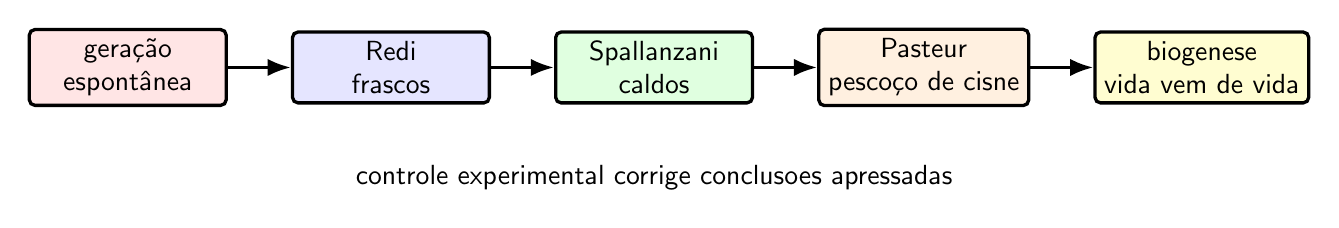
\begin{tikzpicture}[>=Latex,node distance=0.75cm]
  \tikzstyle{box}=[draw,rounded corners=2pt,very thick,align=center,minimum width=2.5cm,minimum height=0.75cm]
  \node[box,fill=red!10] (ge) {geração\\espontânea};
  \node[box,fill=blue!10,right=0.8cm of ge] (redi) {Redi\\frascos};
  \node[box,fill=green!12,right=0.8cm of redi] (spal) {Spallanzani\\caldos};
  \node[box,fill=orange!12,right=0.8cm of spal] (past) {Pasteur\\pescoço de cisne};
  \node[box,fill=yellow!18,right=0.8cm of past] (bio) {biogenese\\vida vem de vida};
  \draw[very thick,->] (ge) -- (redi);
  \draw[very thick,->] (redi) -- (spal);
  \draw[very thick,->] (spal) -- (past);
  \draw[very thick,->] (past) -- (bio);
  \node[align=center,below=0.65cm of spal] {controle experimental corrige conclusoes apressadas};
\end{tikzpicture}
\end{document}
